\documentclass{ximera}

\graphicspath{{./}{thePythagoreanTheorem/}{deMoivreSavesTheDay/}{complexNumbersFromDifferentAngles/}}

\usepackage{tikz}
\usepackage{tkz-euclide}
\usetkzobj{all}
\tikzstyle geometryDiagrams=[ultra thick,color=blue!50!black]
\newcommand{\tri}{\triangle}
\renewcommand{\l}{\ell}
\renewcommand{\P}{\mathcal{P}}
\newcommand{\R}{\mathbb{R}}
\newcommand{\Q}{\mathbb{Q}}

\newcommand{\Z}{\mathbb Z}

\renewcommand{\vec}{\mathbf}
\renewcommand{\d}{\,d}



%% Egyptian symbols

\usepackage{multido}
\newcommand{\egmil}[1]{\multido{\i=1+1}{#1}{
\includegraphics[scale=.1]{egyptian/egypt_person.pdf}\hspace{0.5mm}}}
\newcommand{\eghuntho}[1]{\multido{\i=1+1}{#1}{
\includegraphics[scale=.1]{egyptian/egypt_fish.pdf}\hspace{0.5mm}}}
\newcommand{\egtentho}[1]{\multido{\i=1+1}{#1}{
\includegraphics[scale=.1]{egyptian/egypt_finger.pdf}\hspace{0.5mm}}}
\newcommand{\egtho}[1]{\multido{\i=1+1}{#1}{
\includegraphics[scale=.1]{egyptian/egypt_lotus.pdf}\hspace{0.5mm}}}
\newcommand{\eghun}[1]{\multido{\i=1+1}{#1}{
\includegraphics[scale=.1]{egyptian/egypt_scroll.pdf}\hspace{0.5mm}}}
\newcommand{\egten}[1]{\multido{\i=1+1}{#1}{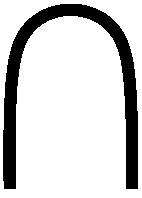
\includegraphics[scale=.1]{egyptian/egypt_heel.pdf}\hspace{0.5mm}}}
\newcommand{\egone}[1]{\multido{\i=1+1}{#1}{
\includegraphics[scale=.1]{egyptian/egypt_stroke.pdf}\hspace{0.5mm}}}
\newcommand{\egyptify}[7]{
 \multido{\i=1+1}{#1}{
\includegraphics[scale=.1]{egyptian/egypt_person.pdf}\hspace{0.5mm}}
 \multido{\i=1+1}{#2}{
\includegraphics[scale=.1]{egyptian/egypt_fish.pdf}\hspace{0.5mm}}
 \multido{\i=1+1}{#3}{
\includegraphics[scale=.1]{egyptian/egypt_finger.pdf}\hspace{0.5mm}}
 \multido{\i=1+1}{#4}{
\includegraphics[scale=.1]{egyptian/egypt_lotus.pdf}\hspace{0.5mm}}
 \multido{\i=1+1}{#5}{
\includegraphics[scale=.1]{egyptian/egypt_scroll.pdf}\hspace{0.5mm}}
 \multido{\i=1+1}{#6}{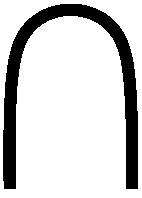
\includegraphics[scale=.1]{egyptian/egypt_heel.pdf}\hspace{0.5mm}}
 \multido{\i=1+1}{#7}{
\includegraphics[scale=.1]{egyptian/egypt_stroke.pdf}\hspace{0.5mm}}
 \hspace{.5mm}
}




\title{The binomial theorem and $\pi$}
\begin{document}
\begin{abstract}
In this activity we investigate a generalization of the binomial theorem and its connection to an approximation of $\pi$.
\end{abstract}
\maketitle


\begin{question}
The binomial theorem states
\[
(a+b)^n = \sum_{k=0}^n \binom{n}{k} a^{n-k}b^k.
\]
Why would we be interested in this? 
\end{question}

\begin{question}
Newton says
\[
(1+x)^r = \sum_{k=0}^\infty \left(\frac{x^k}{k!} \prod_{\l = 0}^{k-1}(r-\l)\right).
\]
How did Newton come up with this? Hint: Calculus!
\end{question}

Now we're going to use this to approximate $\pi$.

\begin{question}
Come up with a function of $x$ for the semicircle of radius $1/2$ centered at $(1/2,0)$. 
\end{question}

\begin{question}
Use Newton's binomial theorem to show your function above is equal to: 
\[
x^{1/2} - \frac{x^{3/2}}{2} - \frac{x^{5/2}}{8} - \frac{x^{7/2}}{16}   - \frac{5x^{9/2}}{128}  - \frac{7x^{11/2}}{256} - \cdots
\]
\end{question}

\begin{question}
Use calculus to compute the area of the shaded region:
\begin{image}
\begin{tikzpicture}[geometryDiagrams]
\begin{axis}[
            ymin=-.05,ymax=.6,
            xmin=-.1,xmax=1.1,
            unit vector ratio*=1 1 1,
            %axis lines =left,
            clip=false,
            every axis y label/.style={at=(current axis.above origin),anchor=south},
            every axis x label/.style={at=(current axis.right of origin),anchor=west},
            xtick={.25, .5, 1},
            xticklabels={$\frac{1}{4}$, $\frac{1}{2}$, $1$},     
            axis lines =middle, xlabel=$x$, ylabel=$y$,
          ]
          \addplot [draw=none,fill=blue!50!white, smooth, domain=(2*pi/3:pi)] ({.5*cos(deg(x))+.5},{.5*sin(deg(x))})\closedcycle;
          \addplot [very thick, smooth, domain=(0:pi)] ({.5*cos(deg(x))+.5},{.5*sin(deg(x))});          
\end{axis}
\end{tikzpicture}
\end{image}
\end{question}

\begin{question}
Use proportional reasoning to compute the area of the sector below:
\begin{image}
\begin{tikzpicture}[geometryDiagrams]
\begin{axis}[
            ymin=-.05,ymax=.6,
            xmin=-.1,xmax=1.1,
            unit vector ratio*=1 1 1,
            %axis lines =left,
            clip=false,
            every axis y label/.style={at=(current axis.above origin),anchor=south},
            every axis x label/.style={at=(current axis.right of origin),anchor=west},
            xtick={.25, .5, 1},
            xticklabels={$\frac{1}{4}$, $\frac{1}{2}$, $1$},     
            axis lines =middle, xlabel=$x$, ylabel=$y$,
          ]
          \addplot [draw=none, fill=blue!50!white,smooth, domain=(2*pi/3:pi)] ({.5*cos(deg(x))+.5},{.5*sin(deg(x))})\closedcycle;
          \addplot [draw=none,fill=blue!50!white] plot coordinates {(.5, 0) (.25,.433)}\closedcycle; %% triangle          
          \addplot [very thick, smooth, domain=(0:pi)] ({.5*cos(deg(x))+.5},{.5*sin(deg(x))});          
\end{axis}
\end{tikzpicture}
\end{image}
\end{question}

\begin{question}
Use the previous problem, along with the area of a certain 30-60-90
right triangle to give a different computation of the area below.
\begin{image}
\begin{tikzpicture}[geometryDiagrams]
\begin{axis}[
            ymin=-.05,ymax=.6,
            xmin=-.1,xmax=1.1,
            unit vector ratio*=1 1 1,
            %axis lines =left,
            clip=false,
            every axis y label/.style={at=(current axis.above origin),anchor=south},
            every axis x label/.style={at=(current axis.right of origin),anchor=west},
            xtick={.25, .5, 1},
            xticklabels={$\frac{1}{4}$, $\frac{1}{2}$, $1$},     
            axis lines =middle, xlabel=$x$, ylabel=$y$,
          ]
          \addplot [draw=none,fill=blue!50!white, smooth, domain=(2*pi/3:pi)] ({.5*cos(deg(x))+.5},{.5*sin(deg(x))})\closedcycle;
          \addplot [very thick, smooth, domain=(0:pi)] ({.5*cos(deg(x))+.5},{.5*sin(deg(x))});          
\end{axis}
\end{tikzpicture}
\end{image}
\end{question}


\begin{question}
Use your work from above to give an approximation of $\pi$.
\end{question}
\end{document}
